%----------------------------------------------------------------------------------------
%    PACKAGES AND THEMES
%----------------------------------------------------------------------------------------
\documentclass[aspectratio=169,xcolor=dvipsnames]{beamer}
\makeatletter
\def\input@path{{../BeamerTemplate/theme/}}
\makeatother
\usetheme{CleanEasy}
\usepackage[utf8]{inputenc}
\usepackage{lmodern}
\usepackage[T1]{fontenc}
\usepackage{fix-cm}
\usepackage{amsmath}
\usepackage{mathtools}
\usepackage{listings}
\usepackage{xcolor}
\usepackage{hyperref}
\usepackage{graphicx}
\usepackage{booktabs}
\usepackage{tikz}
\usetikzlibrary{positioning, shapes, arrows, calc, decorations.pathreplacing, arrows.meta, backgrounds, patterns, overlay-beamer-styles}
\usepackage{etoolbox}

%----------------------------------------------------------------------------------------
%    LAYOUT CONFIGURATION
%----------------------------------------------------------------------------------------
\input{../BeamerTemplate/configs/configs}

%----------------------------------------------------------------------------------------
%    TITLE PAGE CONFIGURATION
%----------------------------------------------------------------------------------------
\title{Linked Lists}
\subtitle{Nodes Connected via Pointers for Flexible Insertions/Deletions}
\author{Minseok Jeon}
\institute{DGIST}
\date{\today}

\begin{document}

\begin{frame}
  \titlepage
\end{frame}

\begin{frame}{Outline}
  \tableofcontents
\end{frame}

% Introduction
\section{Introduction}

\begin{frame}{What is a Linked List?}
  \begin{block}{Definition}
    A linear data structure where elements (nodes) are connected via pointers, allowing dynamic memory allocation and flexible insertions/deletions.
  \end{block}

  \vspace{0.3cm}
  \textbf{Key Characteristics:}
  \begin{itemize}
    \item Non-contiguous memory storage
    \item Dynamic size (grows and shrinks at runtime)
    \item Each node contains data and pointer(s) to next/previous node(s)
    \item No random access (must traverse from head)
  \end{itemize}

  \vspace{0.3cm}
  \textbf{Why Learn Linked Lists?}
  \begin{itemize}
    \item Foundation for stacks, queues, and other data structures
    \item Efficient insertions/deletions at known positions
    \item Understanding pointers and dynamic memory
    \item Common in interviews and real-world systems
  \end{itemize}
\end{frame}

% Types of Linked Lists
\section{Types of Linked Lists}

\subsection{Singly Linked List}

\begin{frame}{Singly Linked List}
  \begin{columns}
    \begin{column}{0.5\textwidth}
      \textbf{Structure:}
      \begin{itemize}
        \item Each node: data + next pointer
        \item Traversal: Forward only
        \item Memory: 1 pointer per node
      \end{itemize}

      \vspace{0.3cm}
      \textbf{Advantages:}
      \begin{itemize}
        \item \checkmark Simple implementation
        \item \checkmark Less memory overhead
        \item \checkmark Efficient forward traversal
      \end{itemize}

      \vspace{0.3cm}
      \textbf{Disadvantages:}
      \begin{itemize}
        \item $\times$ No backward traversal
        \item $\times$ Delete needs previous node
        \item $\times$ No direct tail access
      \end{itemize}
    \end{column}

    \begin{column}{0.5\textwidth}
      \begin{center}
        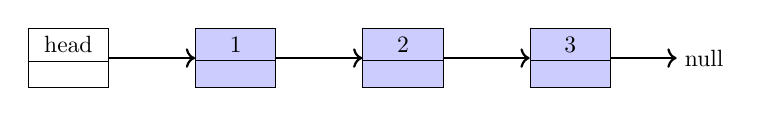
\begin{tikzpicture}[scale=0.85, every node/.style={scale=0.85}]
          \node[draw, rectangle split, rectangle split parts=2, minimum width=1.2cm] (head) at (0, 0) {
            \nodepart{one} head
            \nodepart{two}
          };

          \node[draw, rectangle split, rectangle split parts=2, minimum width=1.2cm, fill=blue!20] (n1) at (2.5, 0) {
            \nodepart{one} 1
            \nodepart{two}
          };

          \node[draw, rectangle split, rectangle split parts=2, minimum width=1.2cm, fill=blue!20] (n2) at (5, 0) {
            \nodepart{one} 2
            \nodepart{two}
          };

          \node[draw, rectangle split, rectangle split parts=2, minimum width=1.2cm, fill=blue!20] (n3) at (7.5, 0) {
            \nodepart{one} 3
            \nodepart{two}
          };

          \node (null) at (9.5, 0) {null};

          \draw[->, thick] (head) -- (n1);
          \draw[->, thick] (n1) -- (n2);
          \draw[->, thick] (n2) -- (n3);
          \draw[->, thick] (n3) -- (null);
        \end{tikzpicture}
      \end{center}

      \vspace{0.5cm}
      \textbf{Visual: head $\to$ [1|$\to$] $\to$ [2|$\to$] $\to$ [3|null]}
    \end{column}
  \end{columns}
\end{frame}

\begin{frame}[fragile]{Singly Linked List: Implementation}
\begin{lstlisting}[language=Python, basicstyle=\tiny\ttfamily]
class Node:
    def __init__(self, data):
        self.data = data
        self.next = None

class SinglyLinkedList:
    def __init__(self):
        self.head = None

    def append(self, data):
        new_node = Node(data)
        if not self.head:
            self.head = new_node
            return

        current = self.head
        while current.next:
            current = current.next
        current.next = new_node

    def display(self):
        elements = []
        current = self.head
        while current:
            elements.append(current.data)
            current = current.next
        return elements
\end{lstlisting}
\end{frame}

\subsection{Doubly Linked List}

\begin{frame}{Doubly Linked List}
  \begin{columns}
    \begin{column}{0.5\textwidth}
      \textbf{Structure:}
      \begin{itemize}
        \item Each node: data + next + prev pointers
        \item Traversal: Both directions
        \item Memory: 2 pointers per node
      \end{itemize}

      \vspace{0.3cm}
      \textbf{Advantages:}
      \begin{itemize}
        \item \checkmark Bidirectional traversal
        \item \checkmark Easier deletion (no prev needed)
        \item \checkmark Can traverse from tail
      \end{itemize}

      \vspace{0.3cm}
      \textbf{Disadvantages:}
      \begin{itemize}
        \item $\times$ More memory (2 pointers)
        \item $\times$ More complex implementation
        \item $\times$ Extra pointer maintenance
      \end{itemize}
    \end{column}

    \begin{column}{0.5\textwidth}
      \begin{center}
        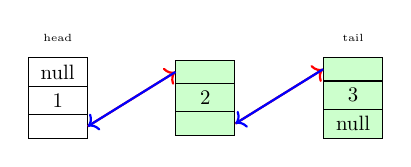
\begin{tikzpicture}[scale=0.75, every node/.style={scale=0.75}]
          \node[draw, rectangle split, rectangle split parts=3, minimum width=1cm] (n1) at (0, 0) {
            \nodepart{one} null
            \nodepart{two} 1
            \nodepart{three}
          };

          \node[draw, rectangle split, rectangle split parts=3, minimum width=1cm, fill=green!20] (n2) at (2.5, 0) {
            \nodepart{one}
            \nodepart{two} 2
            \nodepart{three}
          };

          \node[draw, rectangle split, rectangle split parts=3, minimum width=1cm, fill=green!20] (n3) at (5, 0) {
            \nodepart{one}
            \nodepart{two} 3
            \nodepart{three} null
          };

          \draw[->, thick, red] (n1.three east) -- (n2.one west);
          \draw[<-, thick, blue] (n1.three east) -- (n2.one west);

          \draw[->, thick, red] (n2.three east) -- (n3.one west);
          \draw[<-, thick, blue] (n2.three east) -- (n3.one west);

          \node[above=0.1cm of n1] {\tiny head};
          \node[above=0.1cm of n3] {\tiny tail};
        \end{tikzpicture}
      \end{center}

      \vspace{0.5cm}
      \textbf{Visual:} \\
      head $\to$ [null|1|$\to$] $\leftrightarrow$ [$\leftarrow$|2|$\to$] $\leftrightarrow$ [$\leftarrow$|3|null] $\leftarrow$ tail
    \end{column}
  \end{columns}
\end{frame}

\begin{frame}[fragile]{Doubly Linked List: Implementation}
\begin{lstlisting}[language=Python, basicstyle=\tiny\ttfamily]
class DNode:
    def __init__(self, data):
        self.data = data
        self.next = None
        self.prev = None

class DoublyLinkedList:
    def __init__(self):
        self.head = None
        self.tail = None

    def append(self, data):
        new_node = DNode(data)
        if not self.head:
            self.head = self.tail = new_node
            return

        new_node.prev = self.tail
        self.tail.next = new_node
        self.tail = new_node

    def delete(self, node):
        if node.prev:
            node.prev.next = node.next
        else:
            self.head = node.next

        if node.next:
            node.next.prev = node.prev
        else:
            self.tail = node.prev
\end{lstlisting}
\end{frame}

\subsection{Circular Linked List}

\begin{frame}{Circular Linked List}
  \begin{columns}
    \begin{column}{0.5\textwidth}
      \textbf{Structure:}
      \begin{itemize}
        \item Last node points to first (cycle)
        \item Can be singly or doubly circular
        \item No natural end/null pointer
      \end{itemize}

      \vspace{0.3cm}
      \textbf{Advantages:}
      \begin{itemize}
        \item \checkmark Traverse from any node
        \item \checkmark Round-robin scheduling
        \item \checkmark No null checks
      \end{itemize}

      \vspace{0.3cm}
      \textbf{Disadvantages:}
      \begin{itemize}
        \item $\times$ Risk of infinite loops
        \item $\times$ Complex termination
        \item $\times$ Harder to detect end
      \end{itemize}
    \end{column}

    \begin{column}{0.5\textwidth}
      \begin{center}
        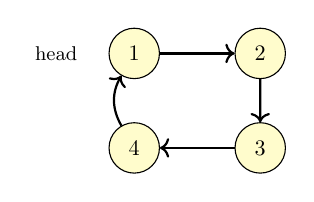
\begin{tikzpicture}[scale=0.8, every node/.style={scale=0.8}]
          \node[draw, circle, minimum size=0.8cm, fill=yellow!20] (n1) at (0, 1.5) {1};
          \node[draw, circle, minimum size=0.8cm, fill=yellow!20] (n2) at (2, 1.5) {2};
          \node[draw, circle, minimum size=0.8cm, fill=yellow!20] (n3) at (2, 0) {3};
          \node[draw, circle, minimum size=0.8cm, fill=yellow!20] (n4) at (0, 0) {4};

          \draw[->, thick] (n1) -- (n2);
          \draw[->, thick] (n2) -- (n3);
          \draw[->, thick] (n3) -- (n4);
          \draw[->, thick, bend left=30] (n4) to (n1);

          \node[left=0.3cm of n1] {\small head};
        \end{tikzpicture}
      \end{center}

      \vspace{0.3cm}
      \textbf{Use Cases:}
      \begin{itemize}
        \item Round-robin CPU scheduling
        \item Music playlists (repeat mode)
        \item Buffer management
      \end{itemize}
    \end{column}
  \end{columns}
\end{frame}

\begin{frame}{Comparison Table}
  \begin{table}
    \centering
    \begin{tabular}{lccc}
      \hline
      \textbf{Feature} & \textbf{Singly} & \textbf{Doubly} & \textbf{Circular} \\
      \hline
      Memory/node & 1 pointer & 2 pointers & 1-2 pointers \\
      Backward traversal & No & Yes & No (singly) \\
      Delete with node & Need prev & $O(1)$ & Need prev \\
      Use case & Simple lists & Undo/redo & Round-robin \\
      \hline
    \end{tabular}
  \end{table}
\end{frame}

% Head/Tail Pointers and Sentinels
\section{Head/Tail Pointers \& Sentinels}

\begin{frame}{Head and Tail Pointers}
  \begin{columns}
    \begin{column}{0.5\textwidth}
      \textbf{Head Pointer Only:}
      \begin{itemize}
        \item Append: $O(n)$ (traverse to end)
        \item Prepend: $O(1)$
        \item Simpler, less memory
      \end{itemize}

      \vspace{0.3cm}
      \textbf{Head + Tail Pointers:}
      \begin{itemize}
        \item Append: $O(1)$ (direct tail access)
        \item Prepend: $O(1)$
        \item Both ends accessible
        \item Perfect for queues
      \end{itemize}
    \end{column}

    \begin{column}{0.5\textwidth}
      \textbf{Benefits of Tail Pointer:}
      \begin{itemize}
        \item \checkmark $O(1)$ append instead of $O(n)$
        \item \checkmark Efficient queue implementation
        \item \checkmark Direct access to last element
      \end{itemize}

      \vspace{0.3cm}
      \textbf{Trade-offs:}
      \begin{itemize}
        \item Extra pointer to maintain
        \item Must update on append/delete
        \item Small memory overhead
      \end{itemize}
    \end{column}
  \end{columns}
\end{frame}

\begin{frame}[fragile]{Optimized List with Tail}
\begin{lstlisting}[language=Python, basicstyle=\small\ttfamily]
class OptimizedList:
    def __init__(self):
        self.head = None
        self.tail = None

    def append(self, data):
        # O(1) with tail pointer
        new_node = Node(data)
        if not self.head:
            self.head = self.tail = new_node
            return

        self.tail.next = new_node
        self.tail = new_node

    def prepend(self, data):
        # O(1)
        new_node = Node(data)
        new_node.next = self.head
        self.head = new_node
        if not self.tail:
            self.tail = new_node
\end{lstlisting}
\end{frame}

\begin{frame}{Sentinel (Dummy) Nodes}
  \begin{block}{Concept}
    Use dummy nodes at head (and optionally tail) to eliminate edge cases for empty lists
  \end{block}

  \vspace{0.3cm}
  \textbf{Benefits:}
  \begin{itemize}
    \item \checkmark Eliminates null checks for empty list
    \item \checkmark Simplifies insertion/deletion code
    \item \checkmark No special cases needed
    \item \checkmark Cleaner, more uniform code
  \end{itemize}

  \vspace{0.3cm}
  \textbf{Trade-offs:}
  \begin{itemize}
    \item $\times$ Extra memory for sentinel(s)
    \item $\times$ Slightly more complex initialization
    \item $\times$ Must skip sentinels during traversal
  \end{itemize}
\end{frame}

\begin{frame}{Sentinel Visualization}
  \begin{center}
    \textbf{Without Sentinel:}
    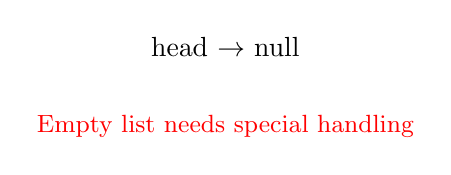
\begin{tikzpicture}[scale=0.8]
      \node (head) at (0, 1) {head $\to$ null};
      \node[below=0.5cm of head, font=\small, red] {Empty list needs special handling};
    \end{tikzpicture}

    \vspace{0.5cm}
    \textbf{With Sentinels (Doubly Linked):}
    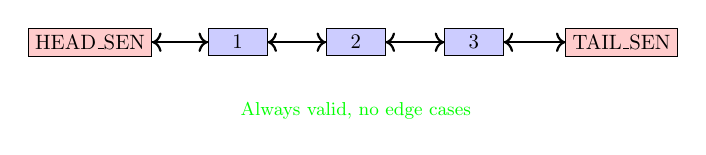
\begin{tikzpicture}[scale=0.75, every node/.style={scale=0.75}]
      \node[draw, rectangle, minimum width=1.5cm, fill=red!20] (hs) at (0, 0) {HEAD\_SEN};
      \node[draw, rectangle, minimum width=1cm, fill=blue!20] (n1) at (2.5, 0) {1};
      \node[draw, rectangle, minimum width=1cm, fill=blue!20] (n2) at (4.5, 0) {2};
      \node[draw, rectangle, minimum width=1cm, fill=blue!20] (n3) at (6.5, 0) {3};
      \node[draw, rectangle, minimum width=1.5cm, fill=red!20] (ts) at (9, 0) {TAIL\_SEN};

      \draw[->, thick] (hs) -- (n1);
      \draw[->, thick] (n1) -- (n2);
      \draw[->, thick] (n2) -- (n3);
      \draw[->, thick] (n3) -- (ts);

      \draw[<-, thick] (hs) -- (n1);
      \draw[<-, thick] (n1) -- (n2);
      \draw[<-, thick] (n2) -- (n3);
      \draw[<-, thick] (n3) -- (ts);

      \node[below=0.5cm of n2, font=\small, green] {Always valid, no edge cases};
    \end{tikzpicture}
  \end{center}
\end{frame}

\begin{frame}[fragile]{Sentinel Implementation}
\begin{lstlisting}[language=Python, basicstyle=\tiny\ttfamily]
class DoublyLinkedListWithSentinel:
    def __init__(self):
        self.head_sentinel = DNode(None)
        self.tail_sentinel = DNode(None)
        self.head_sentinel.next = self.tail_sentinel
        self.tail_sentinel.prev = self.head_sentinel

    def insert_before(self, node, data):
        # Always valid, no edge cases
        new_node = DNode(data)
        new_node.prev = node.prev
        new_node.next = node
        node.prev.next = new_node
        node.prev = new_node

    def delete(self, node):
        # Always valid, no edge cases
        node.prev.next = node.next
        node.next.prev = node.prev

    def is_empty(self):
        return self.head_sentinel.next == self.tail_sentinel
\end{lstlisting}
\end{frame}

% Insertion and Deletion Complexities
\section{Insertion \& Deletion Complexities}

\begin{frame}{Insertion Operations}
  \begin{columns}
    \begin{column}{0.5\textwidth}
      \textbf{Insert at Beginning (Prepend):}
      \begin{itemize}
        \item Create new node
        \item Point to current head
        \item Update head
        \item Time: $O(1)$
      \end{itemize}

      \vspace{0.3cm}
      \textbf{Insert at End (Append):}
      \begin{itemize}
        \item Without tail: $O(n)$ (traverse)
        \item With tail: $O(1)$ (direct)
      \end{itemize}
    \end{column}

    \begin{column}{0.5\textwidth}
      \textbf{Insert at Position $i$:}
      \begin{itemize}
        \item Traverse to position $i-1$
        \item Create new node
        \item Update pointers
        \item Time: $O(i)$
      \end{itemize}

      \vspace{0.3cm}
      \textbf{Insert After Given Node:}
      \begin{itemize}
        \item Have node reference
        \item Create new node
        \item Update pointers
        \item Time: $O(1)$
      \end{itemize}
    \end{column}
  \end{columns}
\end{frame}

\begin{frame}[fragile]{Insertion Examples}
\begin{lstlisting}[language=Python, basicstyle=\tiny\ttfamily]
def prepend(self, data):
    """Insert at beginning - O(1)"""
    new_node = Node(data)
    new_node.next = self.head
    self.head = new_node

def append_fast(self, data):
    """Insert at end with tail - O(1)"""
    new_node = Node(data)
    if not self.tail:
        self.head = self.tail = new_node
    else:
        self.tail.next = new_node
        self.tail = new_node

def insert_at(self, index, data):
    """Insert at position i - O(i)"""
    if index == 0:
        self.prepend(data)
        return

    current = self.head
    for _ in range(index - 1):
        if not current:
            raise IndexError("Index out of bounds")
        current = current.next

    new_node = Node(data)
    new_node.next = current.next
    current.next = new_node
\end{lstlisting}
\end{frame}

\begin{frame}{Deletion Operations}
  \begin{columns}
    \begin{column}{0.5\textwidth}
      \textbf{Delete First Node:}
      \begin{itemize}
        \item Move head to next
        \item Time: $O(1)$
      \end{itemize}

      \vspace{0.3cm}
      \textbf{Delete Last Node:}
      \begin{itemize}
        \item Singly: $O(n)$ (find second-to-last)
        \item Doubly with tail: $O(1)$
      \end{itemize}

      \vspace{0.3cm}
      \textbf{Delete Node with Value:}
      \begin{itemize}
        \item Search for node: $O(n)$
        \item Update pointers: $O(1)$
        \item Total: $O(n)$
      \end{itemize}
    \end{column}

    \begin{column}{0.5\textwidth}
      \textbf{Delete Given Node:}
      \begin{itemize}
        \item Singly: Need previous node
        \item Doubly: $O(1)$ with node reference
      \end{itemize}

      \vspace{0.3cm}
      \textbf{Key Insight:}
      \begin{itemize}
        \item Doubly linked lists excel at deletion
        \item Direct node access $\to$ $O(1)$ delete
        \item Singly linked requires traversal
      \end{itemize}
    \end{column}
  \end{columns}
\end{frame}

\begin{frame}{Complexity Summary Table}
  \begin{table}
    \centering
    \small
    \begin{tabular}{lccc}
      \hline
      \textbf{Operation} & \textbf{Singly (no tail)} & \textbf{Singly (tail)} & \textbf{Doubly (tail)} \\
      \hline
      Prepend & $O(1)$ & $O(1)$ & $O(1)$ \\
      Append & $O(n)$ & $O(1)$ & $O(1)$ \\
      Insert at $i$ & $O(i)$ & $O(i)$ & $O(\min(i, n-i))$ \\
      Delete first & $O(1)$ & $O(1)$ & $O(1)$ \\
      Delete last & $O(n)$ & $O(n)$ & $O(1)$ \\
      Delete at $i$ & $O(i)$ & $O(i)$ & $O(\min(i, n-i))$ \\
      Search & $O(n)$ & $O(n)$ & $O(n)$ \\
      Access by index & $O(i)$ & $O(i)$ & $O(\min(i, n-i))$ \\
      \hline
    \end{tabular}
  \end{table}
\end{frame}

% Reversal and Middle Finding
\section{Reversal \& Middle Finding}

\begin{frame}{Reverse a Linked List: Iterative}
  \textbf{Algorithm:}
  \begin{enumerate}
    \item Initialize prev = None, current = head
    \item While current not None:
    \begin{itemize}
      \item Save next\_node = current.next
      \item Reverse: current.next = prev
      \item Move prev = current
      \item Move current = next\_node
    \end{itemize}
    \item Update head = prev
  \end{enumerate}

  \vspace{0.3cm}
  \textbf{Complexity:}
  \begin{itemize}
    \item Time: $O(n)$ - single pass
    \item Space: $O(1)$ - constant space
  \end{itemize}
\end{frame}

\begin{frame}{Reverse Visualization}
  \begin{center}
    \textbf{Before:}
    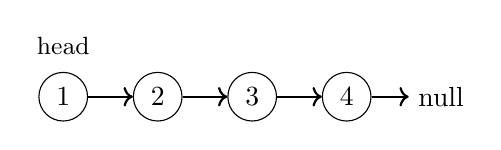
\begin{tikzpicture}[scale=0.8]
      \node[draw, circle] (n1) at (0, 0) {1};
      \node[draw, circle] (n2) at (1.5, 0) {2};
      \node[draw, circle] (n3) at (3, 0) {3};
      \node[draw, circle] (n4) at (4.5, 0) {4};
      \node (null) at (6, 0) {null};

      \draw[->, thick] (n1) -- (n2);
      \draw[->, thick] (n2) -- (n3);
      \draw[->, thick] (n3) -- (n4);
      \draw[->, thick] (n4) -- (null);

      \node[above=0.1cm of n1] {\small head};
    \end{tikzpicture}

    \vspace{0.5cm}
    \textbf{After:}
    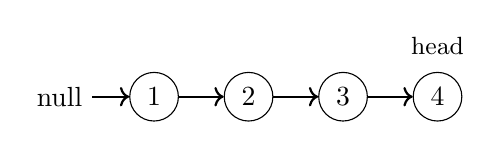
\begin{tikzpicture}[scale=0.8]
      \node (null) at (0, 0) {null};
      \node[draw, circle] (n1) at (1.5, 0) {1};
      \node[draw, circle] (n2) at (3, 0) {2};
      \node[draw, circle] (n3) at (4.5, 0) {3};
      \node[draw, circle] (n4) at (6, 0) {4};

      \draw[<-, thick] (n1) -- (null);
      \draw[<-, thick] (n2) -- (n1);
      \draw[<-, thick] (n3) -- (n2);
      \draw[<-, thick] (n4) -- (n3);

      \node[above=0.1cm of n4] {\small head};
    \end{tikzpicture}
  \end{center}
\end{frame}

\begin{frame}[fragile]{Reverse Implementation}
\begin{lstlisting}[language=Python, basicstyle=\small\ttfamily]
def reverse_iterative(self):
    """Reverse linked list iteratively"""
    prev = None
    current = self.head

    while current:
        next_node = current.next  # Save next
        current.next = prev       # Reverse pointer
        prev = current            # Move prev forward
        current = next_node       # Move current forward

    self.head = prev
    # Time: O(n), Space: O(1)

def reverse_recursive(self, node):
    """Reverse linked list recursively"""
    if not node or not node.next:
        self.head = node
        return node

    rest = self.reverse_recursive(node.next)
    node.next.next = node  # Reverse pointer
    node.next = None

    return rest
    # Time: O(n), Space: O(n) for recursion stack
\end{lstlisting}
\end{frame}

\begin{frame}{Find Middle of Linked List}
  \textbf{Two-Pointer (Slow-Fast) Technique:}
  \begin{itemize}
    \item Use two pointers: slow and fast
    \item Slow moves one step at a time
    \item Fast moves two steps at a time
    \item When fast reaches end, slow is at middle
  \end{itemize}

  \vspace{0.3cm}
  \textbf{Complexity:}
  \begin{itemize}
    \item Time: $O(n)$ - single pass
    \item Space: $O(1)$ - two pointers only
  \end{itemize}

  \vspace{0.3cm}
  \textbf{Advantages:}
  \begin{itemize}
    \item No need to count nodes first
    \item Single traversal
    \item Works for odd and even length lists
  \end{itemize}
\end{frame}

\begin{frame}{Find Middle: Visualization}
  \begin{center}
    \textbf{List: 1 $\to$ 2 $\to$ 3 $\to$ 4 $\to$ 5}

    \vspace{0.3cm}
    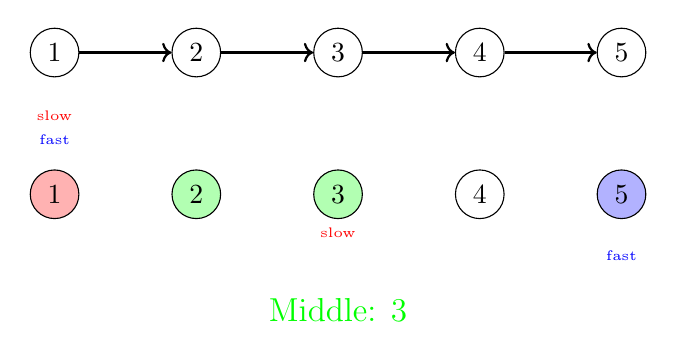
\begin{tikzpicture}[scale=0.9]
      \node[draw, circle] (n1) at (0, 2) {1};
      \node[draw, circle] (n2) at (2, 2) {2};
      \node[draw, circle] (n3) at (4, 2) {3};
      \node[draw, circle] (n4) at (6, 2) {4};
      \node[draw, circle] (n5) at (8, 2) {5};

      \draw[->, thick] (n1) -- (n2);
      \draw[->, thick] (n2) -- (n3);
      \draw[->, thick] (n3) -- (n4);
      \draw[->, thick] (n4) -- (n5);

      % Initial
      \node[below=0.3cm of n1, red] {\tiny slow};
      \node[below=0.6cm of n1, blue] {\tiny fast};

      % After iterations
      \node[draw, circle, fill=red!30] at (0, 0) {1};
      \node[draw, circle, fill=green!30] at (2, 0) {2};
      \node[draw, circle, fill=green!30] at (4, 0) {3};
      \node[draw, circle] at (6, 0) {4};
      \node[draw, circle, fill=blue!30] at (8, 0) {5};

      \node[below=0.3cm of {(4, 0)}, red] {\tiny slow};
      \node[below=0.6cm of {(8, 0)}, blue] {\tiny fast};

      \node[below=1.2cm of {(4, 0)}, green, font=\large] {Middle: 3};
    \end{tikzpicture}
  \end{center}
\end{frame}

\begin{frame}[fragile]{Middle Finding \& Cycle Detection}
\begin{lstlisting}[language=Python, basicstyle=\tiny\ttfamily]
def find_middle(self):
    """Find middle using slow-fast pointers"""
    if not self.head:
        return None

    slow = fast = self.head

    while fast and fast.next:
        slow = slow.next
        fast = fast.next.next

    return slow  # Time: O(n), Space: O(1)

def has_cycle(self):
    """Detect cycle using Floyd's algorithm"""
    if not self.head:
        return False

    slow = fast = self.head

    while fast and fast.next:
        slow = slow.next
        fast = fast.next.next

        if slow == fast:
            return True  # Cycle detected

    return False

def find_kth_from_end(self, k):
    """Find k-th node from end"""
    fast = slow = self.head

    # Move fast k steps ahead
    for _ in range(k):
        if not fast:
            return None
        fast = fast.next

    # Move both until fast reaches end
    while fast:
        slow = slow.next
        fast = fast.next

    return slow
\end{lstlisting}
\end{frame}

% Comparison with Arrays
\section{Comparison with Arrays}

\begin{frame}{Linked Lists vs Arrays}
  \begin{table}
    \centering
    \small
    \begin{tabular}{lcc}
      \hline
      \textbf{Operation} & \textbf{Array} & \textbf{Linked List} \\
      \hline
      Random access & $O(1)$ & $O(n)$ \\
      Sequential access & $O(n)$ & $O(n)$ \\
      Insert at beginning & $O(n)$ & $O(1)$ \\
      Insert at end & $O(1)$ amortized & $O(1)$ with tail \\
      Insert at position $i$ & $O(n)$ & $O(i)$ \\
      Delete at beginning & $O(n)$ & $O(1)$ \\
      Delete at end & $O(1)$ & $O(n)$ singly, $O(1)$ doubly \\
      Search & $O(n)$ or $O(\log n)$ & $O(n)$ \\
      \hline
    \end{tabular}
  \end{table}
\end{frame}

\begin{frame}{Memory Layout Comparison}
  \begin{columns}
    \begin{column}{0.5\textwidth}
      \textbf{Array:}
      \begin{itemize}
        \item Contiguous memory
        \item Address: base + i $\times$ sizeof(element)
        \item Better cache locality
        \item No pointer overhead
      \end{itemize}

      \vspace{0.3cm}
      \begin{center}
        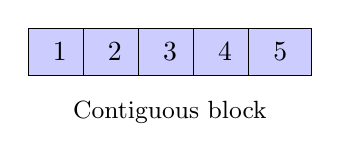
\begin{tikzpicture}[scale=0.7]
          \foreach \x/\val in {0/1, 1/2, 2/3, 3/4, 4/5} {
            \node[draw, rectangle, minimum width=0.8cm, minimum height=0.6cm, fill=blue!20] at (\x*1, 0) {\val};
          }
          \node[below=0.5cm of {(2, 0)}] {\small Contiguous block};
        \end{tikzpicture}
      \end{center}
    \end{column}

    \begin{column}{0.5\textwidth}
      \textbf{Linked List:}
      \begin{itemize}
        \item Scattered nodes
        \item Follow pointers
        \item Poor cache locality
        \item Pointer overhead
      \end{itemize}

      \vspace{0.3cm}
      \begin{center}
        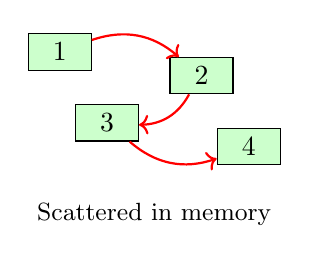
\begin{tikzpicture}[scale=0.6]
          \node[draw, rectangle, minimum width=0.8cm, fill=green!20] (n1) at (0, 1) {1};
          \node[draw, rectangle, minimum width=0.8cm, fill=green!20] (n2) at (3, 0.5) {2};
          \node[draw, rectangle, minimum width=0.8cm, fill=green!20] (n3) at (1, -0.5) {3};
          \node[draw, rectangle, minimum width=0.8cm, fill=green!20] (n4) at (4, -1) {4};

          \draw[->, thick, red] (n1) to[bend left] (n2);
          \draw[->, thick, red] (n2) to[bend left] (n3);
          \draw[->, thick, red] (n3) to[bend right] (n4);

          \node[below=1.2cm of {(2, 0)}] {\small Scattered in memory};
        \end{tikzpicture}
      \end{center}
    \end{column}
  \end{columns}
\end{frame}

\begin{frame}{Advantages \& Disadvantages}
  \begin{columns}
    \begin{column}{0.5\textwidth}
      \textbf{Arrays Advantages:}
      \begin{itemize}
        \item \checkmark $O(1)$ random access
        \item \checkmark Better cache locality
        \item \checkmark Less memory overhead
        \item \checkmark Binary search possible
        \item \checkmark Better for iteration
      \end{itemize}

      \vspace{0.3cm}
      \textbf{When to Use Arrays:}
      \begin{itemize}
        \item Frequent random access
        \item Data size known
        \item Memory locality important
        \item Need sorting/searching
        \item Iteration primary operation
      \end{itemize}
    \end{column}

    \begin{column}{0.5\textwidth}
      \textbf{Linked Lists Advantages:}
      \begin{itemize}
        \item \checkmark $O(1)$ insert/delete at known position
        \item \checkmark No wasted space
        \item \checkmark No element shifting
        \item \checkmark Easy split/merge
        \item \checkmark No reallocation
      \end{itemize}

      \vspace{0.3cm}
      \textbf{When to Use Linked Lists:}
      \begin{itemize}
        \item Frequent insertions/deletions
        \item Unknown/variable size
        \item No random access needed
        \item Implementing stacks/queues
        \item Need to split/merge
      \end{itemize}
    \end{column}
  \end{columns}
\end{frame}

% Memory Overhead and Locality
\section{Memory Overhead \& Locality}

\begin{frame}{Memory Overhead Analysis}
  \textbf{Example: 5 integers}

  \vspace{0.3cm}
  \begin{itemize}
    \item \textbf{Array:}
    \begin{itemize}
      \item Memory: 5 $\times$ 4 bytes = 20 bytes (data only)
      \item Small overhead for array metadata
    \end{itemize}

    \vspace{0.2cm}
    \item \textbf{Singly Linked List:}
    \begin{itemize}
      \item Per node: 4 bytes (int) + 8 bytes (pointer) = 12 bytes
      \item Total: 5 $\times$ 12 = 60 bytes
      \item Overhead: \textbf{200\% more} than array!
    \end{itemize}

    \vspace{0.2cm}
    \item \textbf{Doubly Linked List:}
    \begin{itemize}
      \item Per node: 4 bytes (int) + 16 bytes (2 pointers) = 20 bytes
      \item Total: 5 $\times$ 20 = 100 bytes
      \item Overhead: \textbf{400\% more} than array!
    \end{itemize}
  \end{itemize}

  \vspace{0.3cm}
  \begin{alertblock}{Key Insight}
    Linked lists have significant memory overhead due to pointers
  \end{alertblock}
\end{frame}

\begin{frame}{Cache Locality Impact}
  \begin{columns}
    \begin{column}{0.5\textwidth}
      \textbf{Array (Good Locality):}
      \begin{itemize}
        \item Contiguous layout: [1][2][3][4][5]
        \item Cache line (64 bytes): loads multiple elements
        \item Sequential access $\to$ cache-friendly
        \item Fast iteration
      \end{itemize}

      \vspace{0.3cm}
      \textbf{Performance:}
      \begin{itemize}
        \item Most accesses hit cache (L1/L2)
        \item Prefetching effective
        \item Typical: 1-4 ns per element
      \end{itemize}
    \end{column}

    \begin{column}{0.5\textwidth}
      \textbf{Linked List (Poor Locality):}
      \begin{itemize}
        \item Scattered: [1|$\to$] ... [2|$\to$] ... [3|$\to$] ...
        \item Cache line: only one node
        \item Pointer chasing $\to$ cache misses
        \item Slow iteration
      \end{itemize}

      \vspace{0.3cm}
      \textbf{Performance:}
      \begin{itemize}
        \item Frequent cache misses
        \item Prefetching ineffective
        \item Typical: 5-10x slower than array
      \end{itemize}
    \end{column}
  \end{columns}

  \vspace{0.3cm}
  \begin{block}{Real-World Impact}
    For iteration over 1 million elements, linked lists can be 5-10x slower due to cache misses
  \end{block}
\end{frame}

\begin{frame}{Optimization Techniques}
  \textbf{Improving Linked List Performance:}

  \vspace{0.3cm}
  \begin{enumerate}
    \item \textbf{Memory Pools:}
    \begin{itemize}
      \item Allocate nodes from contiguous pool
      \item Better cache locality
      \item Reduces fragmentation
    \end{itemize}

    \vspace{0.2cm}
    \item \textbf{Unrolled Linked Lists:}
    \begin{itemize}
      \item Store multiple elements per node
      \item Array-like access within node
      \item Balance between linked list and array
    \end{itemize}

    \vspace{0.2cm}
    \item \textbf{Skip Lists:}
    \begin{itemize}
      \item Add express lanes for faster search
      \item $O(\log n)$ search instead of $O(n)$
      \item Probabilistic data structure
    \end{itemize}

    \vspace{0.2cm}
    \item \textbf{XOR Linked Lists:}
    \begin{itemize}
      \item Store XOR of prev and next addresses
      \item Save one pointer per node
      \item More complex but space-efficient
    \end{itemize}
  \end{enumerate}
\end{frame}

% Real-World Applications
\section{Real-World Applications}

\begin{frame}{Application 1: Stack \& Queue Implementation}
  \begin{columns}
    \begin{column}{0.5\textwidth}
      \textbf{Stack (LIFO):}
      \begin{itemize}
        \item Push: $O(1)$ at head
        \item Pop: $O(1)$ from head
        \item Simple, efficient
      \end{itemize}

      \vspace{0.3cm}
      \textbf{Operations:}
      \begin{itemize}
        \item push(x): Add to head
        \item pop(): Remove from head
        \item peek(): View head
      \end{itemize}
    \end{column}

    \begin{column}{0.5\textwidth}
      \textbf{Queue (FIFO):}
      \begin{itemize}
        \item Enqueue: $O(1)$ at tail
        \item Dequeue: $O(1)$ from head
        \item Need head and tail pointers
      \end{itemize}

      \vspace{0.3cm}
      \textbf{Operations:}
      \begin{itemize}
        \item enqueue(x): Add to tail
        \item dequeue(): Remove from head
        \item front(): View head
      \end{itemize}
    \end{column}
  \end{columns}

  \vspace{0.3cm}
  \begin{block}{Why Linked Lists?}
    Both ends accessible in $O(1)$, dynamic size, no reallocation
  \end{block}
\end{frame}

\begin{frame}{Application 2: Browser History}
  \textbf{Back/Forward Navigation:}
  \begin{itemize}
    \item Use doubly linked list
    \item Current page = current node
    \item Back button: current = current.prev
    \item Forward button: current = current.next
    \item Visit new page: add node after current, clear forward history
  \end{itemize}

  \vspace{0.3cm}
  \begin{center}
    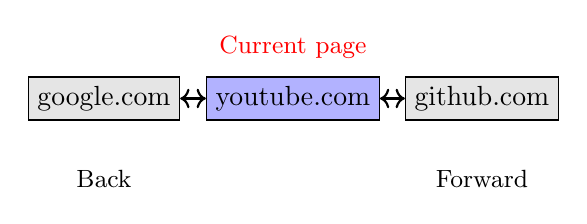
\begin{tikzpicture}[scale=0.8]
      \node[draw, rectangle, fill=gray!20] (p1) at (0, 0) {google.com};
      \node[draw, rectangle, fill=blue!30] (p2) at (3, 0) {youtube.com};
      \node[draw, rectangle, fill=gray!20] (p3) at (6, 0) {github.com};

      \draw[<->, thick] (p1) -- (p2);
      \draw[<->, thick] (p2) -- (p3);

      \node[above=0.1cm of p2, red] {\small Current page};

      \node[below=0.5cm of p1, font=\small] {Back};
      \node[below=0.5cm of p3, font=\small] {Forward};
    \end{tikzpicture}
  \end{center}
\end{frame}

\begin{frame}{Application 3: Music Playlist}
  \textbf{Circular Linked List for Playlists:}
  \begin{itemize}
    \item Last song points to first (repeat mode)
    \item Current song = current node
    \item Next song: current = current.next
    \item Previous song: traverse or use doubly circular
    \item Add/remove songs dynamically
  \end{itemize}

  \vspace{0.3cm}
  \begin{center}
    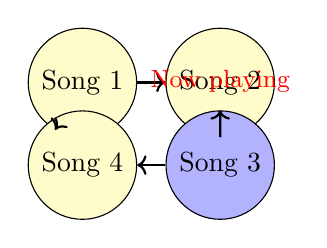
\begin{tikzpicture}[scale=0.7]
      \node[draw, circle, fill=yellow!20] (s1) at (0, 1.5) {Song 1};
      \node[draw, circle, fill=yellow!20] (s2) at (2.5, 1.5) {Song 2};
      \node[draw, circle, fill=blue!30] (s3) at (2.5, 0) {Song 3};
      \node[draw, circle, fill=yellow!20] (s4) at (0, 0) {Song 4};

      \draw[->, thick] (s1) -- (s2);
      \draw[->, thick] (s2) -- (s3);
      \draw[->, thick] (s3) -- (s4);
      \draw[->, thick, bend left=30] (s4) to (s1);

      \node[above=0.1cm of s3, red] {\small Now playing};
    \end{tikzpicture}
  \end{center}
\end{frame}

\begin{frame}{Application 4: Undo/Redo Functionality}
  \textbf{Text Editor Undo/Redo:}
  \begin{itemize}
    \item Use doubly linked list of actions
    \item Current = current action
    \item Undo: current = current.prev, revert action
    \item Redo: current = current.next, apply action
    \item New action: add after current, clear redo history
  \end{itemize}

  \vspace{0.3cm}
  \begin{center}
    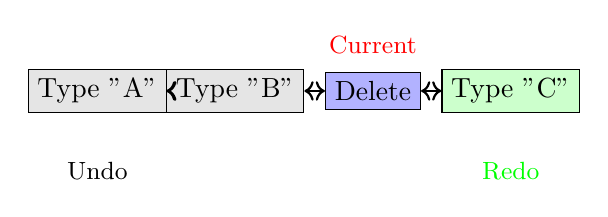
\begin{tikzpicture}[scale=0.7]
      \node[draw, rectangle, fill=gray!20] (a1) at (0, 0) {Type "A"};
      \node[draw, rectangle, fill=gray!20] (a2) at (2.5, 0) {Type "B"};
      \node[draw, rectangle, fill=blue!30] (a3) at (5, 0) {Delete};
      \node[draw, rectangle, fill=green!20] (a4) at (7.5, 0) {Type "C"};

      \draw[<->, thick] (a1) -- (a2);
      \draw[<->, thick] (a2) -- (a3);
      \draw[<->, thick] (a3) -- (a4);

      \node[above=0.1cm of a3, red] {\small Current};
      \node[below=0.5cm of a1, font=\small] {Undo};
      \node[below=0.5cm of a4, font=\small, green] {Redo};
    \end{tikzpicture}
  \end{center}
\end{frame}

\begin{frame}{Application 5: LRU Cache}
  \textbf{Least Recently Used Cache:}
  \begin{itemize}
    \item Doubly linked list + hash table
    \item List ordered by recency (head = most recent, tail = least recent)
    \item Hash table: key $\to$ node (for $O(1)$ access)
    \item Get: move accessed node to head
    \item Put: add to head, if full, remove tail
  \end{itemize}

  \vspace{0.3cm}
  \textbf{Complexity:}
  \begin{itemize}
    \item Get: $O(1)$ (hash lookup + move to head)
    \item Put: $O(1)$ (hash insert + add to head)
  \end{itemize}

  \vspace{0.3cm}
  \textbf{Use Cases:}
  \begin{itemize}
    \item Browser caching
    \item Database query cache
    \item Operating system page replacement
  \end{itemize}
\end{frame}

\begin{frame}{Other Real-World Applications}
  \begin{enumerate}
    \item \textbf{Operating Systems:}
    \begin{itemize}
      \item Process scheduling queues (ready, waiting)
      \item Memory management (free lists)
      \item File system directory entries
      \item Device driver I/O queues
    \end{itemize}

    \vspace{0.2cm}
    \item \textbf{Hash Table Chaining:}
    \begin{itemize}
      \item Each bucket is a linked list
      \item Handle collisions efficiently
      \item Dynamic size per bucket
    \end{itemize}

    \vspace{0.2cm}
    \item \textbf{Symbol Tables:}
    \begin{itemize}
      \item Compiler symbol tables
      \item Variable scope management
      \item Function call stack frames
    \end{itemize}

    \vspace{0.2cm}
    \item \textbf{Graph Representations:}
    \begin{itemize}
      \item Adjacency lists for graphs
      \item Each vertex has linked list of neighbors
      \item Space-efficient for sparse graphs
    \end{itemize}
  \end{enumerate}
\end{frame}

% Summary
\section{Summary}

\begin{frame}{Key Takeaways}
  \textbf{Types of Linked Lists:}
  \begin{itemize}
    \item Singly: Simple, one-way traversal
    \item Doubly: Bidirectional, easier deletion
    \item Circular: No end, round-robin scheduling
  \end{itemize}

  \vspace{0.3cm}
  \textbf{Optimization Techniques:}
  \begin{itemize}
    \item Tail pointer: $O(1)$ append
    \item Sentinel nodes: Eliminate edge cases
    \item Two-pointer: Efficient middle finding, cycle detection
  \end{itemize}

  \vspace{0.3cm}
  \textbf{Trade-offs:}
  \begin{itemize}
    \item $O(1)$ insertion/deletion at known positions vs $O(n)$ random access
    \item Dynamic size vs memory overhead (pointers)
    \item Flexibility vs poor cache locality
  \end{itemize}
\end{frame}

\begin{frame}{When to Use Linked Lists}
  \textbf{Choose Linked Lists When:}
  \begin{itemize}
    \item Frequent insertions/deletions at arbitrary positions
    \item Size unknown or highly variable
    \item No need for random access
    \item Implementing stacks, queues, or other ADTs
    \item Need to frequently split or merge lists
  \end{itemize}

  \vspace{0.3cm}
  \textbf{Choose Arrays When:}
  \begin{itemize}
    \item Need frequent random access
    \item Size is known or stable
    \item Memory locality is critical
    \item Need to sort or perform binary search
    \item Primarily iterating over elements
  \end{itemize}

  \vspace{0.3cm}
  \begin{alertblock}{Key Principle}
    Choose the data structure that optimizes for your most frequent operations
  \end{alertblock}
\end{frame}

\begin{frame}{Practice Problems}
  \textbf{Essential Linked List Problems:}
  \begin{enumerate}
    \item Reverse a linked list (iterative and recursive)
    \item Detect cycle in linked list (Floyd's algorithm)
    \item Find middle of linked list (two pointers)
    \item Merge two sorted linked lists
    \item Remove n-th node from end
    \item Check if linked list is palindrome
    \item Find intersection of two linked lists
    \item Remove duplicates from sorted/unsorted list
    \item Add two numbers represented as linked lists
    \item Flatten a multilevel doubly linked list
  \end{enumerate}

  \vspace{0.3cm}
  \textbf{Resources:}
  \begin{itemize}
    \item LeetCode: Linked List problems (Easy to Hard)
    \item GeeksforGeeks: Comprehensive linked list articles
    \item Cracking the Coding Interview: Chapter on Linked Lists
  \end{itemize}
\end{frame}

\begin{frame}
  \begin{center}
    {\Huge Thank You!}

    \vspace{1cm}
    {\Large Questions?}

    \vspace{1cm}
    \textit{``A linked list is like a treasure hunt -- each node points you to the next clue!''}

    \vspace{0.5cm}
    \small Master linked lists and you'll understand the power of pointers!
  \end{center}
\end{frame}

\end{document}
